\newcommand{\ajuda}{
\begin{tcolorbox}[colback=blue!5!white,colframe=red!25!blue,title= Comando de Ajuda]
Digite os comandos em \textcolor{red}{Vermelho} para obter a ajuda desejada.\\[5pt]
\textcolor{red}{$\backslash$estruturaDoc} Para ajudá-lo com a estrutura do seu documento; \\[5pt]
\textcolor{red}{$\backslash$upArquivos} Para ajudá-lo com o Upload de arquivos para o overleaf; \\[5pt]
\textcolor{red}{$\backslash$fazerLista} Para ajudá-lo a  fazer uma lista numerada ou não; \\\textcolor{red}{$\backslash$adicionaFormula} Para ajudá-lo a adicionar uma equação matemática numerada ou não; \\[5pt]
\textcolor{red}{$\backslash$adicionaCodigo} Para ajudá-lo na adição de um Código;\\
\textcolor{red}{$\backslash$adicionaQuadro} Para ajudá-lo na adição de um Quadro;\\
\textcolor{red}{$\backslash$adicionaTabela} Para ajudá-lo na adição de uma Tabela;\\
\textcolor{red}{$\backslash$adicionaFig} Para ajudá-lo na adição de uma figura; \\[5pt]
\textcolor{red}{$\backslash$letrasGregas} Para ajudá-lo na adição de caracteres gregos;\\
\textcolor{red}{$\backslash$caracterEspecial} Para ajudá-lo na adição de caracteres especiais;\\
\textcolor{red}{$\backslash$adicionaSigla} Para ajudá-lo na adição de uma Sigla;\\
\textcolor{red}{$\backslash$adicionaSimbolo} Para ajudá-lo na adição de um Simbolo;\\
\textcolor{red}{$\backslash$adicionaPalavraGlossario} Para ajudá-lo na adição de uma Palavra ao Glossário;\\[10pt]
Quando não precisar mais de ajuda, comente a linha \textcolor{blue}{$\backslash$ajuda} \texttt{ - para comentar digite o caracter \% antes do comando. Ex. \textcolor{black!40!white}{\%$\backslash$ajuda}}
\end{tcolorbox}
}

\newcommand{\adicionaFormula}{
\begin{tcolorbox}[colback=blue!5!white,colframe=black!25!pink,title= Comandos básicos utilizados para acrescentar equações numeradas ou não]
\ding{42} Formas de adicionar uma equação não numerada:\\[5pt]
\ding{172} No meio de texto; 
$$\text{texto1} \$\texttt{equação}\$\text{ texto2}$$
Ex. O teorema \$c\^{}2 = a\^{}2 + b\^{}2\$ a seguir $\Rightarrow$  O teorema $c^2 = a^2 + b^2$ a seguir\\[5pt]
\ding{173} Centralizado em linha separada
$$\$\$\text{ equação }\$\$$$
Ex. \$\$\textcolor{blue}{$\backslash$displaystyle $\backslash$sum}\_\{i=1\}\^{}n f\textcolor{blue}{$\backslash$left}(x\_i\textcolor{blue}{$\backslash$right})\$\$ quando compilado
$$\displaystyle \sum_{i=1}^nf\left(x_i\right)$$
\ding{42} Formas de adicionar uma equação numerada:\\[5pt]
\textcolor{blue}{$\backslash$begin}\{equation\} \texttt{ - inicia o ambiente equação}\\
\textcolor{blue}{$\backslash$displaystyle $\backslash$int}\_a\^{}b f(x)dx = F(b) - F(a) \texttt{ - equação}\\
\textcolor{blue}{$\backslash$label}\{eq:cap1eq1\} \texttt{ - rótulo da equação no documento}\\
\textcolor{blue}{$\backslash$end}\{equation\} \texttt{ - finaliza o ambiente equação}\\[10pt]
Quando compilada a equação \ref{eq:cap1eq1} ficaria
\begin{equation}
    \displaystyle \int_a^bf(x)dx=F(b)-F(a)
    \label{eq:cap1eq1}
\end{equation}
\ding{96} necessário no caso de referenciar em outra parte do documento\\
Para não exibir numeração \textcolor{blue}{$\backslash$begin}\{equation*\} $\ldots$ \textcolor{blue}{$\backslash$end}\{equation*\}\\[5pt]
Para a equação à esquerda modifique as configurações no preambulo (antes dos pacotes) \textcolor{blue}{$\backslash$documentclass}[fleqn]\{classe do documento\}
\end{tcolorbox}
}

\newcommand{\estruturaDoc}{
\begin{tcolorbox}[colback=blue!5!white,colframe=black!25!yellow,title= Comandos básico utilizados na estrutura desse documento]
Principais comando utilizados na estrutura hierárquica desse documento:\\[5pt]
\textcolor{blue}{$\backslash$chapter}\{título do capítulo\}\texttt{ - para abreviar no sumário utilize ``$\backslash$chapter[título abreviado]\{título do capítulo\}'' sem aspas}\\
\textcolor{blue}{$\backslash$section}\{título da seção\}\texttt{ - texto do segundo nível}\\
\textcolor{blue}{$\backslash$subsection}\{título da subseção\}\texttt{ - texto do terceiro nível}\\
\textcolor{blue}{$\backslash$subsubsection}\{título do 4\textdegree~ nível\}\\[10pt]
Capítulos, seções, subseções e subsubseções podem ser rotulados, logo abaixo da entrada do capítulo, para eventuais chamadas em outras partes do documento.\\[10pt]
\textcolor{blue}{$\backslash$label}\{sec:introdução\}\texttt{ - exemplo de entrada do rótulo de chamada da introdução}\\[10pt]
\textcolor{blue}{$\backslash$ref}\{sec:introdução\} \texttt{ - quando digitado no documento, faz a referência ao capítulo introdução} 
\end{tcolorbox}
}
\newcommand{\caracterEspecial}{
\begin{tcolorbox}[colback=blue!5!white,colframe=red!25!yellow,title= Comandos para caracteres especiais]
Para adicionar um caracter especial digite um dos comando em \textcolor{blue}{azul} abaixo:\\[5pt]
\begin{tabular}{lclp{3cm}rcl}
\textcolor{blue}{$\backslash$\$}&\texttt{-  para -}&\$&&\textcolor{blue}{$\backslash$\&}&\texttt{-  para -}&\&\\
\textcolor{blue}{$\backslash$\%}&\texttt{-  para -}&\%&&\textcolor{blue}{$\backslash$\#}&\texttt{-  para -}&\#\\
\textcolor{blue}{$\backslash$\_}&\texttt{-  para -}&\_&&\textcolor{blue}{$\backslash$\{}&\texttt{-  para -}&\{\\
\textcolor{blue}{$\backslash$\}}&\texttt{-  para -}&\}&&\textcolor{blue}{$\backslash$\~{}\{\}}&\texttt{-  para -}&\~{}\\
\textcolor{blue}{$\backslash$\^{}\{\}}&\texttt{-  para -}&\^{}&&\textcolor{blue}{\$$\backslash$backslash\$}&\texttt{-  para -}&$\backslash$\\
\end{tabular}
\end{tcolorbox}
}

\newcommand{\letrasGregas}{
\begin{tcolorbox}[colback=blue!5!white,colframe=red!75!yellow,title= Comandos para caracteres gregos]
Para adicionar uma letra grega digite um dos comando em \textcolor{blue}{azul} abaixo:\\[5pt]
\begin{tabular}{lcl}
\textcolor{blue}{$\backslash$alpha} \texttt{-  para a letra \alpha}&&\textcolor{blue}{$\backslash$beta} \texttt{-  para a letra \beta}\\
\textcolor{blue}{$\backslash$gamma} \texttt{-  para a letra \gamma}&&\textcolor{blue}{$\backslash$delta} \texttt{-  para a letra \delta}\\
\textcolor{blue}{$\backslash$epsilon} \texttt{-  para a letra \epsilon}&&\textcolor{blue}{$\backslash$varepsilon} \texttt{-  para a caracter \varepsilon}\\
\textcolor{blue}{$\backslash$zeta} \texttt{-  para a letra \zeta}&&\textcolor{blue}{$\backslash$eta} \texttt{-  para a letra \eta}\\
\textcolor{blue}{$\backslash$theta} \texttt{-  para a letra \theta}&&\textcolor{blue}{$\backslash$vartheta} \texttt{-  para o caracter \vartheta}\\
\textcolor{blue}{$\backslash$iota} \texttt{-  para a letra \iota}&&\textcolor{blue}{$\backslash$kappa} \texttt{-  para a letra \kappa}\\
\textcolor{blue}{$\backslash$lambda} \texttt{-  para a letra \lambda}&&\textcolor{blue}{$\backslash$mu} \texttt{-  para a letra \mu}\\
\textcolor{blue}{$\backslash$nu} \texttt{-  para a letra \nu}&&\textcolor{blue}{$\backslash$xi} \texttt{-  para a letra \xi}\\
\textcolor{blue}{o} \texttt{-  para a letra ômicron}&&\textcolor{blue}{$\backslash$pi} \texttt{-  para a letra \pi}\\
\textcolor{blue}{$\backslash$varpi} \texttt{-  para o caracter \varpi}&&\textcolor{blue}{$\backslash$rho} \texttt{-  para a letra \rho}\\
\textcolor{blue}{$\backslash$varrho} \texttt{-  para o caracter \varrho}&&\textcolor{blue}{$\backslash$sigma} \texttt{-  para a letra \sigma}\\
\textcolor{blue}{$\backslash$varsigma} \texttt{-  para o caracter \varsigma}&&\textcolor{blue}{$\backslash$tau} \texttt{-  para a letra \tau}\\
\textcolor{blue}{$\backslash$upsilon} \texttt{-  para a letra \upsilon}&&\textcolor{blue}{$\backslash$phi} \texttt{-  para a letra \phi}\\
\textcolor{blue}{$\backslash$varphi} \texttt{-  para o caracter \varphi}&&\textcolor{blue}{$\backslash$chi} \texttt{-  para a letra \chi}\\
\textcolor{blue}{$\backslash$psi} \texttt{-  para a letra \psi}&&\textcolor{blue}{$\backslash$omega} \texttt{-  para a letra \omega}
\end{tabular}\\[5pt]
Caracteres Maiúsculos\\
\begin{tabular}{lcl}
\textcolor{blue}{$\backslash$Gamma} \texttt{-  para a letra \Gamma}&&\textcolor{blue}{$\backslash$Delta} \texttt{-  para a letra \Delta}\\
\textcolor{blue}{$\backslash$Theta} \texttt{-  para a letra \Theta}&&\textcolor{blue}{$\backslash$Lambda} \texttt{-  para a letra \Lambda}\\
\textcolor{blue}{$\backslash$Xi} \texttt{-  para a letra \Xi}&&\textcolor{blue}{$\backslash$Pi} \texttt{-  para a letra \Pi}\\
\textcolor{blue}{$\backslash$Sigma} \texttt{-  para a letra \Sigma}&&\textcolor{blue}{$\backslash$Upsilon} \texttt{-  para a letra \Upsilon}\\
\textcolor{blue}{$\backslash$Phi} \texttt{-  para a letra \Phi}&&\textcolor{blue}{$\backslash$Psi} \texttt{-  para a letra \Psi}\\
\textcolor{blue}{$\backslash$Omega} \texttt{-  para a letra \Omega}&&\\
\end{tabular}
\end{tcolorbox}
}



\newcommand{\adicionaFig}{
\begin{tcolorbox}[colback=blue!5!white,colframe=green!75!blue,title= Comando Acrescenta figura, fontlower=\footnotesize]
Para adicionar uma figura no documento siga os passos abaixo:\\[5pt]
\textcolor{blue}{$\backslash$begin}\{figure\}[h!]\\
\texttt{Inicia o ambiente, o ``h!'' significa aqui, ``H'' - Ambos fixam a imagem naquela exata posição do texto}\\
\textcolor{blue}{$\backslash$setstretch\{1.5\}$\backslash$centering$\backslash$footnotesize} \\
\texttt{Configura Rodapé: espaçamento - centralização - tamanho da fonte}\\
\textcolor{blue}{$\backslash$caption}\{texto\}\texttt{ - ``texto'' é a descrição da figura no documento} \\
\textcolor{blue}{$\backslash$begin}\{center\} \texttt{centraliza a imagem}\\
\textcolor{blue}{$\backslash$includegraphics}[tamanho]\{nomeArquivo\}\\
\texttt{ - ``tamanho'' pode ser escalonado(ex. scale=0.5) ou largura(width) e altura(height), ex. width=3cm, height=0.5$\backslash$linewidth.\\
``nome.ext'' todas as imagens devem ser adicionadas na pasta ``imagens''. A ``.ext'' refere-se a extensão da imagem ex. .jpg,.png,etc}\\
\textcolor{blue}{$\backslash$end}\{center\} \texttt{Fim da centralização da Imagem}\\
\textcolor{blue}{$\backslash$label}\{fig:nomedafigura\}\texttt{ - indica como a figura será referenciada no documento}\\
\textcolor{blue}{$\backslash$par} Fonte:  local de origem \texttt{ - indica o local de origem da figura ou quem a produziu}\\
\textcolor{blue}{$\backslash$end}\{figure\}\texttt{ - finaliza o ambiente figure}
\tcblower
\textcolor{blue}{EXEMPLO}\\
$\backslash$begin\{figure\}[H]\\
\tab $\backslash$setstretch\{1.5\}$\backslash$centering$\backslash$footnotesize\\
\tab $\backslash$caption\{Album A Presenca da Gloria da banda Santa Geracao\}\\
\tab $\backslash$begin\{center\}\\
\tab \tab $\backslash$includegraphics[width=0.5$\backslash$textwidth]\{presencaDaGloria.png\}\\
\tab $\backslash$end\{center\}\\
\tab $\backslash$label\{fig:capaPresencaDaGloria\}\\
\tab $\backslash$par Fonte: Google Imagens\\
$\backslash$end\{figure\}\\
\end{tcolorbox}
}

\newcommand{\adicionaQuadro}{
\begin{tcolorbox}[colback=blue!5!white,colframe=green!75!blue,title= Comando Acrescenta Quadro, fontlower=\footnotesize]
Acesse o site: https://www.tablesgenerator.com para produzir um quadro/tabela\\
\textcolor{blue}{$\backslash$begin}\{Quadro\}[H]\texttt{ - inicia o ambiente quadros ``H'' aqui!}\\
\textcolor{blue}{$\backslash$setstretch\{1.5\}$\backslash$centering$\backslash$footnotesize} \\
\texttt{Conf. Rodapé: espaçamento|centralização|tamanho da fonte}\\
\textcolor{blue}{$\backslash$caption}\{texto\}\texttt{ - ``texto'' é a descrição do quadro}\\
\textcolor{blue}{$\backslash$begin}\{center\}\texttt{ - inicia o ambiente centralizar}\\
\textcolor{blue}{$\backslash$begin}\{tabular\}\{|c|c|\}\textcolor{blue}{$\backslash$hline}\texttt{- inicia o ambiente tabular que cria a estrutura do quadro, ``|c|c|'' são duas colunas centralizadas, ``$\backslash$hline'' insere uma linha horizontal}\\
Título Coluna1 \& Título Coluna2 \textcolor{blue}{$\backslash \backslash \backslash$hline}\texttt{ - Texto das colunas ``\&'' separa as colunas}\\
valor1 \& valor2 \textcolor{blue}{$\backslash\backslash \backslash$hline}\texttt{ - valores das colunas para uma linha. Para acrescentar mais linhas insira os valores, separados por \& e finalize com $\backslash\backslash \backslash$hline}\\
\textcolor{blue}{$\backslash$end}\{tabular\}\texttt{ - finaliza o ambiente tabular}\\
\textcolor{blue}{$\backslash$end}\{center\}\texttt{ - finaliza o ambiente centralizar}\\
\textcolor{blue}{$\backslash$label}\{qua:nome\}\texttt{ - insere um rótulo para a chamar o quadro}\\
 \textcolor{blue}{$\backslash$par} Fonte: Elaborado por \texttt{ - indica a fonte do quadro}\\
\textcolor{blue}{$\backslash$end}\{Quadro\}\texttt{ - finaliza o ambiente quadro}
\tcblower
\textcolor{blue}{EXEMPLO}\\
$\backslash$begin\{Quadro\}[H]\\
\tab $\backslash$setstretch\{1.5\}$\backslash$centering$\backslash$footnotesize\\
\tab $\backslash$caption\{Quadro sem sentido.\}\\
\tab $\backslash$begin\{center\}\\
\tab \tab $\backslash$begin\{tabular\}\{|c|c|\}\\
\tab \tab \tab $\backslash$hline\\
\tab \tab \tab Título Coluna \& Título Coluna $\backslash$$\backslash$\\
\tab \tab \tab $\backslash$hline\\
\tab \tab \tab X \& Y $\backslash$$\backslash$\\
\tab \tab \tab $\backslash$hline\\
\tab \tab $\backslash$end\{tabular\}\\
\tab $\backslash$end\{center\}\\
\tab $\backslash$label\{qua:tabela-ssentido\}\\
\tab $\backslash$par Fonte: Elaborado pelo próprio autor.\\
$\backslash$end\{Quadro\}\\
\end{tcolorbox}
}

\newcommand{\adicionaTabela}{
\begin{tcolorbox}[colback=blue!5!white,colframe=green!75!blue,title= Comando Adiciona Tabela, fontupper=\footnotesize, fontlower=\footnotesize]
Acesse o site: https://www.tablesgenerator.com para produzir um quadro/tabela\\
\textcolor{blue}{$\backslash$begin}\{table\}[H] \texttt{ - Inicia o ambiente tabela}\\
\textcolor{blue}{$\backslash$setstretch\{1.5\}$\backslash$centering$\backslash$footnotesize} \\
\texttt{Conf. Rodapé: espaçamento|centralização|tamanho da fonte}\\
\textcolor{blue}{$\backslash$caption}\{texto\}\texttt{ - ``texto'' é a descrição da tabela no documento}\\
\textcolor{blue}{$\backslash$begin}\{center\}\texttt{- inicia o ambiente centralizador da tabela na página}\\
\textcolor{blue}{$\backslash$begin}\{tabular\}\{p\{0.8cm\} crlS[table-format=0.1]\} \texttt{inicia o ambiente tabular}\\
\texttt{formato das colunas: ``p\{valor em \textit{cm}\}'' para coluna de tamanho fixo | ``c'' coluna com texto centralizado | ``r'' texto à direita | ``l'' texto à esquerda}\\
\textcolor{blue}{$\backslash$toprule}\texttt{ - linha superior da tabela}\\
Coluna1 \& coluna2 \textcolor{blue}{$\backslash\backslash$}\texttt{ - texto das colunas | ``\&'' separador dos dados das colunas | padrão usado no cabeçalho e dados}\\
\textcolor{blue}{$\backslash$midrule}\texttt{ - linha abaixo do cabeçalho}\\
\textcolor{blue}{$\backslash$bottomrule}\texttt{ - linha inferior(abaixo) da tabela}\\
\textcolor{blue}{$\backslash$end}\{tabular\}\texttt{ - finalização do ambiente tabular}\\
\textcolor{blue}{$\backslash$end}\{center\}\texttt{ - finalização do ambiente centralizador}\\
\textcolor{blue}{$\backslash$label}\{table:tabelanome\}\texttt{ - insere o rotulo ''table:tabelanome'' para chamar no documento}\\
\textcolor{blue}{$\backslash$par} Fonte: Elaborado por \texttt{ - indica a fonte dos dados da tabela}\\
\textcolor{blue}{$\backslash$end}\{table\}\texttt{ - finalização do ambiente tabela}
\tcblower
$\backslash$begin\{table\}[H]\\
\tab $\backslash$setstretch\{1.5\}$\backslash$centering$\backslash$footnotesize\\
\tab $\backslash$caption\{Cronograma\} \\
\tab $\backslash$begin\{center\} \\
\tab \tab $\backslash$begin\{tabular\}\{p\{7cm\}S[table-format=0.2]\}\\
\tab \tab \tab $\backslash$toprule \\
\tab \tab \tab \{2019\} \& \{Ago\} $\backslash$$\backslash$\\
\tab \tab \tab $\backslash$midrule\\
\tab \tab \tab Revisão bibliográfica  \& X \&  $\backslash$$\backslash$\\
\tab \tab \tab $\backslash$bottomrule\\
\tab \tab $\backslash$end\{tabular\} \\
\tab $\backslash$end\{center\} \\
\tab $\backslash$label\{table:cronograma\} \\
\tab $\backslash$par Fonte: Elaborado pelo próprio autor. \\
$\backslash$end\{table\} \\
\end{tcolorbox}
}

\newcommand{\upArquivos}{
\begin{tcolorbox}[colback=blue!5!white,colframe=green!75!blue,title= Ajuda para fazer Upload de arquivos]
Para fazer o upload de um arquivo siga os passos ilustrados abaixo:\\[5pt]
\ding{46} Na janela de arquivos do Overleaf, navegue até a pasta imagens \ding{202};\\
\ding{46} clique no icone de upload \ding{202};\\
\ding{46} navegue na pasta do computador até o local do arquivo \ding{203};\\
\ding{46} arraste o arquivo para a janela de upload \ding{204}.\\[5pt]
\begin{tikzpicture}
\node[] at (0.3, -5.8)  (t1) {\large\ding{202}};
\node[] at (5.3, -5.8)  (t3) {\large\ding{204}};
\node[] at (10.3, -5.8)  (t2) {\large\ding{203}};
\node[] at (0, -4)  (a1)    {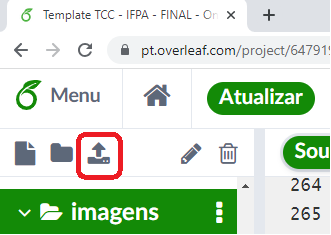
\includegraphics[scale=0.3]{Backup/up1.png}}; 
\node[] at (1, -3.5)  (a2) {
\includegraphics[scale=0.09]{Backup/up3a.png}};
\node[] at (5.5, -4)  (a3) {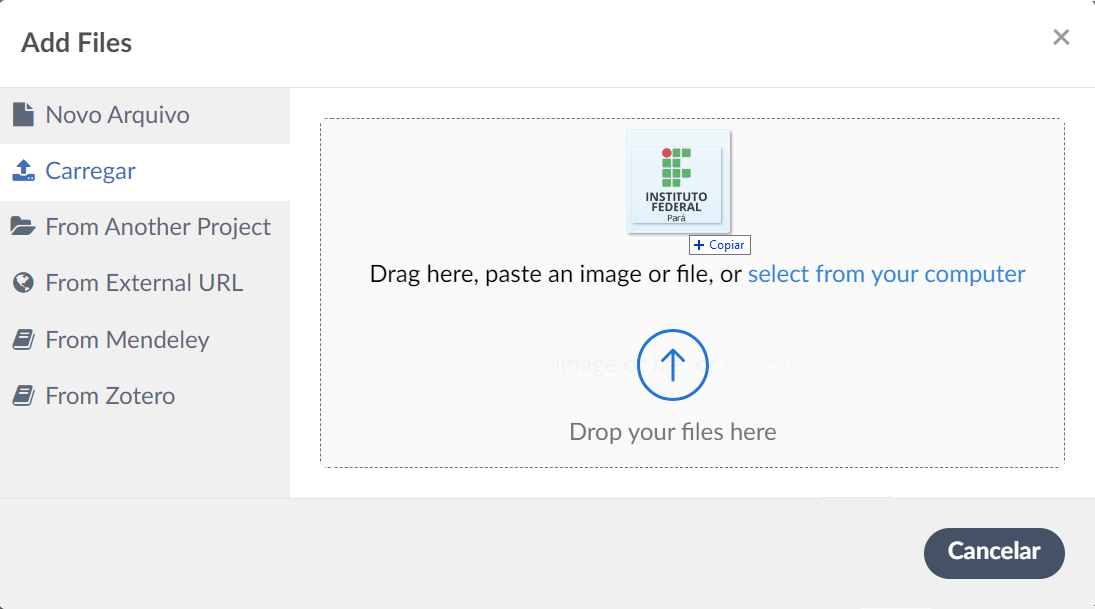
\includegraphics[scale=0.13]{Backup/up2.png}};
\node[] at (10.5, -4)  (a3) {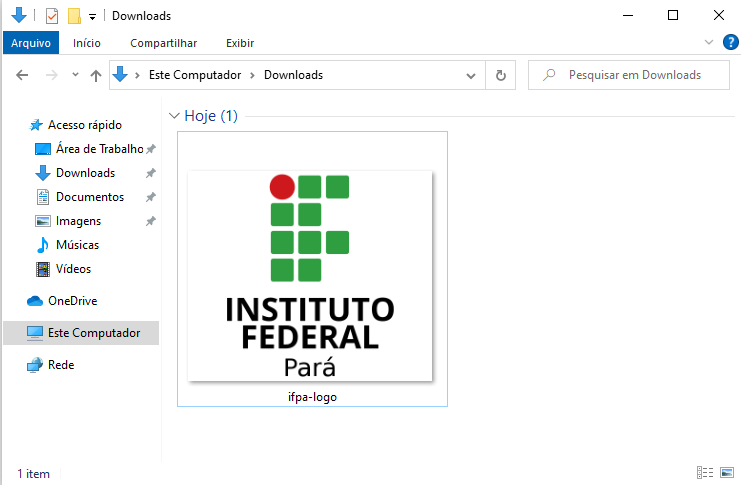
\includegraphics[scale=0.15]{Backup/up4.png}};
\node[] at (8.5, -3)  (a3) {
\includegraphics[scale=0.09]{Backup/up3b.png}};
\end{tikzpicture}
\end{tcolorbox}
}

\newcommand{\fazerLista}{
\begin{tcolorbox}[colback=blue!5!white,colframe=green!75!blue,title= Como criar uma lista numerada ou não]
Para criar uma Lista não numerada siga os passos abaixo:\\[5pt] 
\textcolor{blue}{$\backslash$begin}\{itemize\} \texttt{ - Inicia o ambiente lista}\\
\textcolor{blue}{$\backslash$item} primeiro\\ 
\textcolor{blue}{$\backslash$item} segundo\\
\textcolor{blue}{$\backslash$end}\{itemize\} \texttt{ - Finaliza o ambiente lista}\\[5pt]
\texttt{você deverá digitar o primeiro elemento da sua lista depois do comando  ``$\backslash$item''. Para acrescentar mais itens, após o ``Enter'' digite ``$\backslash$item'' antes do seu texto}
 \begin{multicols}{2}
Sua lista terá a aparência a seguir
\begin{itemize}
\item primeiro
\item segundo
\end{itemize}

\columnbreak
mudando o rótulo: \\\textcolor{blue}{$\backslash$begin}\{itemize\}[label=\textcolor{blue}{$\backslash$ding}\{42\}]
\begin{itemize}[label=\ding{42}]
\item primeiro
\item segundo
\end{itemize}
\end{multicols}
\textcolor{green!70!black}{Para mais rótulos, no Google procure \textit{pifont table}}\\[5pt]
Para criar uma Lista não numerada\\
\textcolor{blue}{$\backslash$begin}\{enumerate\} \texttt{ - Inicia o ambiente lista enumerada}\\
\textcolor{blue}{$\backslash$item} primeiro\\ 
\textcolor{blue}{$\backslash$item} segundo\\
\textcolor{blue}{$\backslash$end}\{enumerate\} \texttt{ - Finaliza o ambiente lista enumerada}
\begin{multicols}{2}
Sua lista terá a aparência a seguir
\begin{enumerate}
\item primeiro
\item segundo
\end{enumerate}

\columnbreak
mudando o rótulo: \\\textcolor{blue}{$\backslash$begin}\{enumerate\}[label=(\textcolor{blue}{$\backslash$alph*})]
\begin{enumerate}[label=(\alph*)]
\item primeiro
\item segundo
\end{enumerate}
\end{multicols}
\end{tcolorbox}
}

\newcommand{\adicionaCodigo}{
\begin{tcolorbox}[colback=blue!5!white,colframe=green!75!blue,title= Comando Adiciona Código, fontlower=\footnotesize]
Para adicionar código de uma linguagem de programação, siga os passos abaixo:\\[5pt] 
\textcolor{blue}{$\backslash$begin}\{lstlisting\}[language=\{\textcolor{blue}{NomeLinguagem}\}, caption=\{\textcolor{blue}{Nome Do Código}\}] \\ \texttt{ - Inicia o ambiente de código \\ Informa a Linguagem de Programação \\ Informa o título do código}\\
Código da Linguagem de Programação\\
\textcolor{blue}{$\backslash$end}\{lstlisting\}\texttt{ - finalização do ambiente de código}
\tcblower
\textcolor{blue}{EXEMPLO}\\
$\backslash$begin\{lstlisting\}[language=Python, caption=HelloWorld]\\
\tab print("Ola, Mundo")\\
$\backslash$end\{lstlisting\}\\
\end{tcolorbox}
}


%% \adicionaSigla
\newcommand{\adicionaSigla}{
\begin{tcolorbox}[colback=blue!5!white,colframe=green!75!blue,title= Comando Adiciona Sigla, fontlower=\footnotesize]
Para adicionar uma Sigla importante ao Texto e que deverá aparecer na \textcolor{blue}{Lista de Siglas e Abreviações}, siga os passos abaixo:\\[5pt] 
\textcolor{blue}{1 - Acesse o arquivo \{Escritor$\backslash$abreviaçõesSiglas.tex\}} \\[5pt]
\textcolor{blue}{EXEMPLO}\\[5pt]
\textcolor{blue}{$\backslash$DeclareAcronym}\{sbc\}\{\\
\texttt{Comando gerador de sigla \{ palavraChaveSigla \}}\\
\tab short = \normalfont{SBC}, \texttt{A Sigla como aparecerá}\\
\tab short-plural = s, \texttt{Sigla no modo plural (adição de s)}\\
\tab long  = Sociedade Brasileira de Computação, \texttt{por Extenso}\\
\tab tag = abbrev \texttt{abbrev - indicativo de SIGLA}\\
\} \texttt{- Fim da declaração de Sigla}\\[5pt]
\textcolor{blue}{2 - Faça referência à Sigla no Texto}
\tcblower
\textcolor{blue}{EXEMPLO}\\
\texttt{Teremos 2 comandos}\\[5pt]
\textcolor{blue}{$\backslash$ac}\{palavraChaveSigla\}\\
\texttt{Usado para mostrar a SIGLA literal}\\
\textcolor{blue}{$\backslash$acl}\{palavraChaveSigla\}\\
\texttt{Usado para mostrar a forma extensa da Sigla}\\
\textcolor{blue}{EXEMPLO}\\[5pt]
$\backslash$ac\{sbc\}\\
$\backslash$acl\{sbc\}\\
\\[5pt]
\textcolor{blue}{SBC}\\
\textcolor{blue}{Sociedade Brasileira de Computação}
\end{tcolorbox}
}


%% \adicionaSimbolo
\newcommand{\adicionaSimbolo}{
\begin{tcolorbox}[colback=blue!5!white,colframe=green!75!blue,title= Comando Adiciona Símbolo, fontlower=\footnotesize]
Para adicionar um Símbolo importante ao texto e que deverá aparecer na \textcolor{blue}{Lista de Símbolos}, siga os passos abaixo:\\[5pt] 
\textcolor{blue}{1 - Acesse o arquivo \{Escritor$\backslash$simbolos.tex\}} \\[5pt]
\textcolor{blue}{EXEMPLO}\\[5pt]
\textcolor{blue}{$\backslash$DeclareAcronym}\{megaByte\}\{\\
\texttt{Comando gerador de símbolo \{ palavraChaveSigla \}}\\
\tab short = \normalfont{MB}, \texttt{O Símbolo como aparecerá}\\
\tab long  = é uma unidade de medida de informação,\\
\tab \texttt{Significado do Símbolo por Extenso}\\
\tab sort  = MB, \texttt{Letra usada para ORDENAR na lista}\\
\tab tag = nomen \texttt{nomen- indicativo de SÍMBOLO}\\
\} \texttt{- Fim da declaração de Símbolo}\\[5pt]
\textcolor{blue}{2 - Faça referência ao Símbolo no Texto}
\tcblower
\textcolor{blue}{EXEMPLO}\\
\texttt{Teremos 2 comandos}\\[5pt]
\textcolor{blue}{$\backslash$ac}\{palavraChaveSigla\}\\
\texttt{Usado para mostrar a SIGLA literal}\\
\textcolor{blue}{$\backslash$acl}\{palavraChaveSigla\}\\
\texttt{Usado para mostrar a forma extensa da Sigla}\\
\textcolor{blue}{EXEMPLO}\\[5pt]
$\backslash$ac\{megaByte\}\\
$\backslash$acl\{megaByte\}\\
\\[5pt]
\textcolor{blue}{MB}\\
\textcolor{blue}{é uma unidade de medida de informação}
\end{tcolorbox}
}

%% \adicionaPalavraGlossario
\newcommand{\adicionaPalavraGlossario}{
\begin{tcolorbox}[colback=blue!5!white,colframe=green!75!blue,title= Comando Adiciona Palavras ao Glossário, fontlower=\footnotesize]
Para adicionar uma Palavra que é importante ao texto e que deverá aparecer no \textcolor{blue}{Glossário}, siga os passos abaixo:\\[5pt] 
\textcolor{blue}{1 - Acesse o arquivo \{Escritor$\backslash$glossario.tex\}} \\[5pt]
\textcolor{blue}{EXEMPLO}\\[5pt]
\textcolor{blue}{$\backslash$newglossaryentry}\{latex\}\{\\
\texttt{Gerador de Palavra do Glossário \{ palavraChaveGlossario \}}\\
\tab name = \{LATEX\}, \texttt{- Palavra como aparecerá no Glossário}\\
\tab text  = \{LaTeX\}, \texttt{- Como aparecerá no texto} \\
\tab sort = \{latex\}, \texttt{- Usado para Ordenar as palavra }\\
\tab description = \{É uma linguagem de marcação especialmente feita para documentos científicos\}, \\
\tab \texttt{Descrição por extenso da palavra - LaTeX}\\
\} \texttt{- Fim da declaração de Palavra do Glossário}\\[5pt]
\textcolor{blue}{2 - Faça referência à Palavra do Glossário no Texto} \\[5pt]
\textcolor{blue}{EXEMPLO}\\[5pt]
\texttt{Teremos 1 comando}\\[5pt]
\textcolor{blue}{$\backslash$gls}\{palavraChaveGlossário\}\\
\texttt{Usado para mostrar o texto da Palavra do Glossário}
\tcblower
\textcolor{blue}{EXEMPLO}\\
$\backslash$gls\{latex\}\\
\\[5pt]
\textcolor{blue}{LaTeX}\\
\end{tcolorbox}
}